\section{Benchmarks and Quality Evidence}
\label{sec:evaluation}
\subsection{A Quality Profile Rather Than a Single Score}
We organize test quality as a profile of complementary properties. \emph{Input validity} asks whether the input satisfies the task's domain constraints. \emph{Executability} asks whether the test can be built and run in the intended environment. \emph{Oracle correctness} asks whether its judgment follows the intended specification. \emph{Defect detection} asks whether it rejects relevant invalid behavior. \emph{Non-rejection} asks whether it accepts permitted behavior. Coverage, stability, maintainability, and cost add further dimensions needed for deployment.

Denominators differ: compilation can cover all attempts, whereas coverage and mutation often use retained tests. Report attempted, executable, accepted, and retained artifacts to expose filtering. Per-test and per-suite results are complementary, since one invalid assertion can cause an otherwise useful suite to reject a correct implementation.

\begin{figure}[t]
\centering
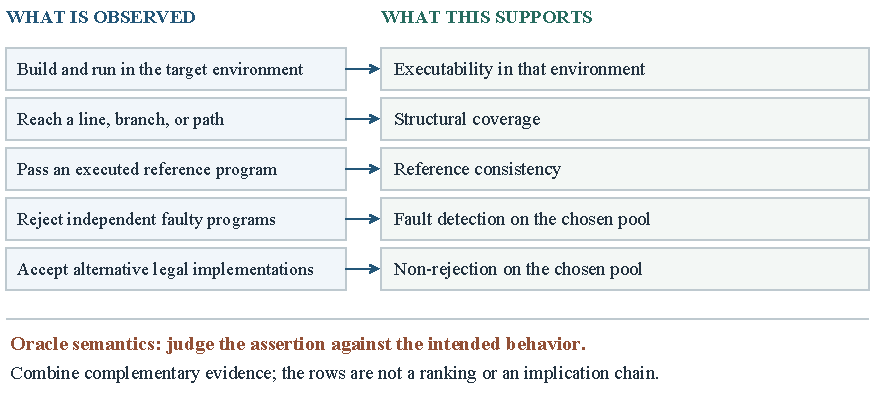
\includegraphics[width=\linewidth]{figures/quality-evidence.pdf}
\caption{Quality evidence supports different conclusions. Each arrow connects an observation to its immediate interpretation. Oracle correctness additionally depends on the intended specification and the validity of the evidence sources. These dimensions are complementary rather than successive levels of one score.}
\Description{Five separate arrows connect successful execution, structural reachability, reference passing, rejection of faulty programs, and acceptance of legal implementations to their corresponding bounded quality claims. No arrows connect these claims into a hierarchy.}
\label{fig:evidence}
\end{figure}

Figure~\ref{fig:evidence} connects each observation to its bounded interpretation. Coverage measures reach; mutation depends on its fault model and test validity; reference passing assumes a suitable reference. Assertion matching measures similarity, code-selection accuracy measures downstream utility, and repeated-run passing measures stability. These signals remain useful at their respective levels.

\subsection{Benchmark Families}
TestGenEval evaluates test generation and completion in real Python repositories~\cite{B01}. TESTEVAL emphasizes test generation for program coverage, including targeted structural objectives~\cite{B02}. Both are relevant to executable testing, but their task construction changes the context and the question being measured. Repository tasks expose dependencies and established tests; structural targets isolate whether generation can reach particular code regions.

SWT-Bench evaluates tests distinguishing buggy software from real-world fixes~\cite{B03}. Patch discrimination requires issue-related failure and acceptance of the fix, but does not characterize every legal implementation.

ULT/PLT studies test generation from real-world functions and examines contamination-related evaluation conditions~\cite{B04}. RESTestBench studies REST API tests generated from natural-language requirements, including requirement precision and SUT feedback~\cite{B05}. These benchmarks expose issues that small function tasks can underrepresent: complex context, ambiguity, dependencies between operations, and the quality of feedback used to revise a test.

Recent empirical work adds complementary evaluation dimensions. A study of real Python bugs compares LLM and human unit tests through fault detection~\cite{E01}. Research under software evolution studies test generation across semantic changes~\cite{E02}. Database testing work investigates flakiness in industrial and open-source settings~\cite{E03}. These studies broaden the target from initial generation quality to the behavior of tests on historical defects, changed software, and repeated executions.

Newer resources isolate further comparison conditions. TC-Bench selects a compact pool of erroneous contest programs through a code--test outcome matrix~\cite{B06}. Its discrimination and rank properties concern that observed pool. MultiFileTest moves evaluation to multi-file projects and distinguishes error-fixing configurations~\cite{B07}. TOGBench covers several oracle forms and reinserts generated oracles into Java tests for compilation, execution, and mutation assessment~\cite{B08}. The latter's repository uses ``false positive'' for erroneous programs that still pass; we retain that operational definition rather than equating it with rejection of legal implementations.

\begin{table}[t]
\caption{Benchmark selection should follow the intended claim. Rows identify primary emphases rather than exhaustive benchmark capabilities.}
\label{tab:benchmarks}
\small
\begin{tabularx}{\linewidth}{@{}p{.22\linewidth}YY@{}}
\toprule
Benchmark family & Useful question & Comparison condition to preserve \\
\midrule
TestGenEval~\cite{B01} & Can tests be constructed in repositories? & Existing tests, dependencies, generation versus completion \\
TESTEVAL~\cite{B02} & Can tests reach structural targets? & Target visibility and coverage denominator \\
SWT-Bench~\cite{B03} & Can tests expose an issue and accept its fix? & Issue information and buggy/fixed execution protocol \\
ULT/PLT~\cite{B04} & How do real functions and leakage conditions affect evaluation? & Dataset construction and model exposure assumptions \\
RESTestBench~\cite{B05} & How do requirements and feedback affect API tests? & Requirement precision and feedback validity \\
TC-Bench~\cite{B06} & Can tests distinguish selected erroneous solutions? & Candidate-pool construction and matrix definition \\
MultiFileTest~\cite{B07} & Can tests use multi-file project context? & Language, repository context, and repair configuration \\
TOGBench~\cite{B08} & Can generated oracles replace diverse Java oracles? & Oracle type, reinsertion, and metric definitions \\
\bottomrule
\end{tabularx}
\end{table}

The benchmark portfolio should follow the claim: repository usability, requirements reasoning, patch discrimination, and independent discovery require different evidence. Scores from unrelated protocols cannot be combined into a method ranking.

\subsection{Implementation State and Metric Interpretation}
Empirical studies increasingly separate tests generated from correct and buggy code. Work on incorrect-code influence and buggy-code misguidance examines how implementation errors affect generated judgments~\cite{E04,E06}. Replacing code with a generated docstring can change that influence, but the docstring remains code-derived~\cite{E06}. The requirements-oracle study instead evaluates requirement agreement separately from agreement with the SUT; its ten Lang-bug cases and repair-derived requirement construction bound the setting~\cite{O12}.

The same distinction qualifies proxy metrics. A replicability study reports that coverage and mutation can inform model comparison in regression settings where code is reasonably assumed correct, while their reliability for detecting existing bugs is weaker~\cite{E05}. Test Wars also illustrates that mutation, coverage, and fault-detection rankings can differ across LLM, search-based, and symbolic approaches~\cite{E08}. These observations support task-specific metric interpretation, rather than discarding structural metrics. The Java-oracle study uses developer-oracle comparison as a correctness proxy and mutation as a detection proxy~\cite{E07}; neither exhausts specification conformance.

Fuzzing adds a related failure-attribution problem. A crash from a generated driver can reflect an invalid API use rather than a reachable product defect. Google's OSS-Fuzz-Gen report examines false-positive mitigation using API constraints and realistic entry-point context~\cite{F09}. Valid input or driver construction, reproduced failure, and confirmed defect should therefore be separate stages of the reporting funnel.

\subsection{Independent Oracle Assessment}
The requirement can be viewed as defining a set of permitted implementations. For an illustrative evaluation, let $\mathcal{P}^{+}$ be independently validated implementations that satisfy the requirement and let $\mathcal{P}^{-}$ be independently constructed faulty implementations. For a test suite $T$, define
\begin{equation}
\mathrm{RejectLegal}(T)=\frac{\sum_{p\in\mathcal{P}^{+}}\mathbf{1}[T(p)=\mathrm{fail}]}{|\mathcal{P}^{+}|},\qquad
\mathrm{DetectFault}(T)=\frac{\sum_{p\in\mathcal{P}^{-}}\mathbf{1}[T(p)=\mathrm{fail}]}{|\mathcal{P}^{-}|}.
\end{equation}
The two quantities measure complementary behavior on finite evaluation pools. They require a nonempty pool of each kind, valid execution environments, and trustworthy pool labels. They are an evaluation recommendation rather than measurements extracted from the reviewed studies. Reporting them together exposes suites that detect many faults by also rejecting permitted behavior. Neither quantity alone proves specification-wide correctness.

Alternative correct algorithms and permissible output choices test whether an oracle encodes unstated implementation details. Faults withheld from training, prompting, and feedback test independent detection. Where executable pools are unavailable, expert scenario assessment should record traceability, applicability, expected behavior, omissions, and assessor disagreement; textual similarity alone does not establish detection.

\subsection{Comparability, Leakage, and Cost}
Comparisons need matched information contracts: requirements-only generation, reference access, and candidate-feedback repair are different settings. Training data, retrieval, existing tests, and evaluation artifacts can cross intended boundaries. Contamination controls should identify the paths they address.

Cost should include model calls, input and output tokens, conventional executions, environment preparation, and human intervention. For trained generators, training cost and deployment cost answer different questions and should be reported separately. For hybrid fuzzers, execution throughput and the reuse of generated infrastructure matter. For agent systems, total calls across all roles matter. An equal-token comparison and an equal-wall-time comparison may favor different designs, so both can be informative when resources permit.

Generation randomness and execution nondeterminism are separate sources of variance. Project-level results, repeated generation, repeated execution, failed attempts, and stopping rules make uncertainty and selection effects assessable.
